\documentclass[a4paper, 11pt]{article}
%%%%%%%%%%%%%%%%%%%%%%%%%%%%%%%%%%%%%%%%%%%%%%%%%%%%%%%%%%%%%%%%%%%%%%%%%%%%%%%
%                                Basic Packages                               %
%%%%%%%%%%%%%%%%%%%%%%%%%%%%%%%%%%%%%%%%%%%%%%%%%%%%%%%%%%%%%%%%%%%%%%%%%%%%%%%

% Gives us multiple colors.
\usepackage[usenames,dvipsnames,pdftex]{xcolor}
% Lets us style link colors.
\usepackage{hyperref}
% Lets us import images and graphics.
\usepackage{graphicx}
% Lets us use figures in floating environments.
\usepackage{float}
% Lets us create multiple columns.
\usepackage{multicol}
% Gives us better math syntax.
\usepackage{amsmath,amsfonts,mathtools,amsthm,amssymb}
% Lets us strikethrough text.
\usepackage{cancel}
% Lets us edit the caption of a figure.
\usepackage{caption}
% Lets us import pdf directly in our tex code.
\usepackage{pdfpages}
% Lets us do algorithm stuff.
\usepackage[ruled,vlined,linesnumbered]{algorithm2e}
% Use a smiley face for our qed symbol.
\usepackage{tikzsymbols}
% \usepackage{fullpage} %%smaller margins
\usepackage[shortlabels]{enumitem}

\setlist[enumerate]{font={\bfseries}} % global settings, for all lists

\usepackage{setspace}
\usepackage[margin=1in, headsep=12pt]{geometry}
\usepackage{wrapfig}
\usepackage{listings}
\usepackage{parskip}

\definecolor{codegreen}{rgb}{0,0.6,0}
\definecolor{codegray}{rgb}{0.5,0.5,0.5}
\definecolor{codepurple}{rgb}{0.58,0,0.82}
\definecolor{backcolour}{rgb}{0.95,0.95,0.95}

\lstdefinestyle{mystyle}{
    backgroundcolor=\color{backcolour},   
    commentstyle=\color{codegreen},
    keywordstyle=\color{magenta},
    numberstyle=\tiny\color{codegray},
    stringstyle=\color{codepurple},
    basicstyle=\ttfamily\footnotesize,
    breakatwhitespace=false,         
    breaklines=true,                 
    captionpos=b,                    
    keepspaces=true,                 
    numbers=left,                    
    numbersep=5pt,                  
    showspaces=false,                
    showstringspaces=false,
    showtabs=false,                  
    tabsize=2,
    numbers=none
}

\lstset{style=mystyle}
\def\class{article}


%%%%%%%%%%%%%%%%%%%%%%%%%%%%%%%%%%%%%%%%%%%%%%%%%%%%%%%%%%%%%%%%%%%%%%%%%%%%%%%
%                                Basic Settings                               %
%%%%%%%%%%%%%%%%%%%%%%%%%%%%%%%%%%%%%%%%%%%%%%%%%%%%%%%%%%%%%%%%%%%%%%%%%%%%%%%

%%%%%%%%%%%%%
%  Symbols  %
%%%%%%%%%%%%%

\let\implies\Rightarrow
\let\impliedby\Leftarrow
\let\iff\Leftrightarrow
\let\epsilon\varepsilon
%%%%%%%%%%%%
%  Tables  %
%%%%%%%%%%%%

\setlength{\tabcolsep}{5pt}
\renewcommand\arraystretch{1.5}

%%%%%%%%%%%%%%
%  SI Unitx  %
%%%%%%%%%%%%%%

\usepackage{siunitx}
\sisetup{locale = FR}

%%%%%%%%%%
%  TikZ  %
%%%%%%%%%%

\usepackage[framemethod=TikZ]{mdframed}
\usepackage{tikz}
\usepackage{tikz-cd}
\usepackage{tikzsymbols}

\usetikzlibrary{intersections, angles, quotes, calc, positioning}
\usetikzlibrary{arrows.meta}

\tikzset{
    force/.style={thick, {Circle[length=2pt]}-stealth, shorten <=-1pt}
}

%%%%%%%%%%%%%%%
%  PGF Plots  %
%%%%%%%%%%%%%%%

\usepackage{pgfplots}
\pgfplotsset{width=10cm, compat=newest}

%%%%%%%%%%%%%%%%%%%%%%%
%  Center Title Page  %
%%%%%%%%%%%%%%%%%%%%%%%

\usepackage{titling}
\renewcommand\maketitlehooka{\null\mbox{}\vfill}
\renewcommand\maketitlehookd{\vfill\null}

%%%%%%%%%%%%%%%%%%%%%%%%%%%%%%%%%%%%%%%%%%%%%%%%%%%%%%%
%  Create a grey background in the middle of the PDF  %
%%%%%%%%%%%%%%%%%%%%%%%%%%%%%%%%%%%%%%%%%%%%%%%%%%%%%%%

\usepackage{eso-pic}
\newcommand\definegraybackground{
    \definecolor{reallylightgray}{HTML}{FAFAFA}
    \AddToShipoutPicture{
        \ifthenelse{\isodd{\thepage}}{
            \AtPageLowerLeft{
                \put(\LenToUnit{\dimexpr\paperwidth-222pt},0){
                    \color{reallylightgray}\rule{222pt}{297mm}
                }
            }
        }
        {
            \AtPageLowerLeft{
                \color{reallylightgray}\rule{222pt}{297mm}
            }
        }
    }
}

%%%%%%%%%%%%%%%%%%%%%%%%
%  Modify Links Color  %
%%%%%%%%%%%%%%%%%%%%%%%%

\hypersetup{
    % Enable highlighting links.
    colorlinks,
    % Change the color of links to blue.
    urlcolor=blue,
    % Change the color of citations to black.
    citecolor={black},
    % Change the color of url's to blue with some black.
    linkcolor={blue!80!black}
}

%%%%%%%%%%%%%%%%%%
% Fix WrapFigure %
%%%%%%%%%%%%%%%%%%

\newcommand{\wrapfill}{\par\ifnum\value{WF@wrappedlines}>0
        \parskip=0pt
        \addtocounter{WF@wrappedlines}{-1}%
        \null\vspace{\arabic{WF@wrappedlines}\baselineskip}%
        \WFclear
    \fi}

%%%%%%%%%%%%%%%%%
% Multi Columns %
%%%%%%%%%%%%%%%%%

\let\multicolmulticols\multicols
\let\endmulticolmulticols\endmulticols

\RenewDocumentEnvironment{multicols}{mO{}}
{%
    \ifnum#1=1
        #2%
    \else % More than 1 column
        \multicolmulticols{#1}[#2]
    \fi
}
{%
    \ifnum#1=1
    \else % More than 1 column
        \endmulticolmulticols
    \fi
}

\newlength{\thickarrayrulewidth}
\setlength{\thickarrayrulewidth}{5\arrayrulewidth}


%%%%%%%%%%%%%%%%%%%%%%%%%%%%%%%%%%%%%%%%%%%%%%%%%%%%%%%%%%%%%%%%%%%%%%%%%%%%%%%
%                           School Specific Commands                          %
%%%%%%%%%%%%%%%%%%%%%%%%%%%%%%%%%%%%%%%%%%%%%%%%%%%%%%%%%%%%%%%%%%%%%%%%%%%%%%%

%%%%%%%%%%%%%%%%%%%%%%%%%%%
%  Initiate New Counters  %
%%%%%%%%%%%%%%%%%%%%%%%%%%%

\newcounter{lecturecounter}

%%%%%%%%%%%%%%%%%%%%%%%%%%
%  Helpful New Commands  %
%%%%%%%%%%%%%%%%%%%%%%%%%%

\makeatletter

\newcommand\resetcounters{
    % Reset the counters for subsection, subsubsection and the definition
    % all the custom environments.
    \setcounter{subsection}{0}
    \setcounter{subsubsection}{0}
    \setcounter{definition0}{0}
    \setcounter{paragraph}{0}
    \setcounter{theorem}{0}
    \setcounter{claim}{0}
    \setcounter{corollary}{0}
    \setcounter{proposition}{0}
    \setcounter{lemma}{0}
    \setcounter{exercise}{0}
    \setcounter{problem}{0}
    
    \setcounter{subparagraph}{0}
    % \@ifclasswith\class{nocolor}{
    %     \setcounter{definition}{0}
    % }{}
}

%%%%%%%%%%%%%%%%%%%%%
%  Lecture Command  %
%%%%%%%%%%%%%%%%%%%%%

\usepackage{xifthen}

% EXAMPLE:
% 1. \lecture{Oct 17 2022 Mon (08:46:48)}{Lecture Title}
% 2. \lecture[4]{Oct 17 2022 Mon (08:46:48)}{Lecture Title}
% 3. \lecture{Oct 17 2022 Mon (08:46:48)}{}
% 4. \lecture[4]{Oct 17 2022 Mon (08:46:48)}{}
% Parameters:
% 1. (Optional) lecture number.
% 2. Time and date of lecture.
% 3. Lecture Title.
\def\@lecture{}
\def\@lectitle{}
\def\@leccount{}
\newcommand\lecture[3]{
    \newpage

    % Check if user passed the lecture title or not.
    \def\@leccount{Lecture #1}
    \ifthenelse{\isempty{#3}}{
        \def\@lecture{Lecture #1}
        \def\@lectitle{Lecture #1}
    }{
        \def\@lecture{Lecture #1: #3}
        \def\@lectitle{#3}
    }

    \setcounter{section}{#1}
    \renewcommand\thesubsection{#1.\arabic{subsection}}
    
    \phantomsection
    \addcontentsline{toc}{section}{\@lecture}
    \resetcounters

    \begin{mdframed}
        \begin{center}
            \Large \textbf{\@leccount}
            
            \vspace*{0.2cm}
            
            \large \@lectitle
            
            
            \vspace*{0.2cm}

            \normalsize #2
        \end{center}
    \end{mdframed}

}

%%%%%%%%%%%%%%%%%%%%
%  Import Figures  %
%%%%%%%%%%%%%%%%%%%%

\usepackage{import}
\pdfminorversion=7

% EXAMPLE:
% 1. \incfig{limit-graph}
% 2. \incfig[0.4]{limit-graph}
% Parameters:
% 1. The figure name. It should be located in figures/NAME.tex_pdf.
% 2. (Optional) The width of the figure. Example: 0.5, 0.35.
\newcommand\incfig[2][1]{%
    \def\svgwidth{#1\columnwidth}
    \import{./figures/}{#2.pdf_tex}
}

\begingroup\expandafter\expandafter\expandafter\endgroup
\expandafter\ifx\csname pdfsuppresswarningpagegroup\endcsname\relax
\else
    \pdfsuppresswarningpagegroup=1\relax
\fi

%%%%%%%%%%%%%%%%%
% Fancy Headers %
%%%%%%%%%%%%%%%%%

\usepackage{fancyhdr}

% Force a new page.
\newcommand\forcenewpage{\clearpage\mbox{~}\clearpage\newpage}

% This command makes it easier to manage my headers and footers.
\newcommand\createintro{
    % Use roman page numbers (e.g. i, v, vi, x, ...)
    \pagenumbering{roman}

    % Display the page style.
    \maketitle
    % Make the title pagestyle empty, meaning no fancy headers and footers.
    \thispagestyle{empty}
    % Create a newpage.
    \newpage

    % Input the intro.tex page if it exists.
    \IfFileExists{intro.tex}{ % If the intro.tex file exists.
        % Input the intro.tex file.
        \textbf{Course}: MATH 16300: Honors Calculus III

\textbf{Section}: 43

\textbf{Professor}: Minjae Park

\textbf{At}: The University of Chicago

\textbf{Quarter}: Spring 2023

\textbf{Course materials}: Calculus by Spivak (4th Edition), Calculus On Manifolds by Spivak

\vspace{1cm}
\textbf{Disclaimer}: This document will inevitably contain some mistakes, both simple typos and serious logical and mathematical errors. Take what you read with a grain of salt as it is made by an undergraduate student going through the learning process himself. If you do find any error, I would really appreciate it if you can let me know by email at \href{mailto:conghungletran@gmail.com}{conghungletran@gmail.com}.

        % Make the pagestyle fancy for the intro.tex page.
        \pagestyle{fancy}

        % Remove the line for the header.
        \renewcommand\headrulewidth{0pt}

        % Remove all header stuff.
        \fancyhead{}

        % Add stuff for the footer in the center.
        % \fancyfoot[C]{
        %   \textit{For more notes like this, visit
        %   \href{\linktootherpages}{\shortlinkname}}. \\
        %   \vspace{0.1cm}
        %   \hrule
        %   \vspace{0.1cm}
        %   \@author, \\
        %   \term: \academicyear, \\
        %   Last Update: \@date, \\
        %   \faculty
        % }

        \newpage
    }{ % If the intro.tex file doesn't exist.
        % Force a \newpageage.
        % \forcenewpage
        \newpage
    }

    % Remove the center stuff we did above, and replace it with just the page
    % number, which is still in roman numerals.
    \fancyfoot[C]{\thepage}
    % Add the table of contents.
    \tableofcontents
    % Force a new page.
    \newpage

    % Move the page numberings back to arabic, from roman numerals.
    \pagenumbering{arabic}
    % Set the page number to 1.
    \setcounter{page}{1}

    % Add the header line back.
    \renewcommand\headrulewidth{0.4pt}
    % In the top right, add the lecture title.
    \fancyhead[R]{\footnotesize \@lecture}
    % In the top left, add the author name.
    \fancyhead[L]{\footnotesize \@author}
    % In the bottom center, add the page.
    \fancyfoot[C]{\thepage}
    % Add a nice gray background in the middle of all the upcoming pages.
    % \definegraybackground
}

\makeatother


%%%%%%%%%%%%%%%%%%%%%%%%%%%%%%%%%%%%%%%%%%%%%%%%%%%%%%%%%%%%%%%%%%%%%%%%%%%%%%%
%                               Custom Commands                               %
%%%%%%%%%%%%%%%%%%%%%%%%%%%%%%%%%%%%%%%%%%%%%%%%%%%%%%%%%%%%%%%%%%%%%%%%%%%%%%%

%%%%%%%%%%%%
%  Circle  %
%%%%%%%%%%%%

\newcommand*\circled[1]{\tikz[baseline= (char.base)]{
        \node[shape=circle,draw,inner sep=1pt] (char) {#1};}
}

%%%%%%%%%%%%%%%%%%%
%  Todo Commands  %
%%%%%%%%%%%%%%%%%%%

% \usepackage{xargs}
% \usepackage[colorinlistoftodos]{todonotes}

% \makeatletter

% \@ifclasswith\class{working}{
%     \newcommandx\unsure[2][1=]{\todo[linecolor=red,backgroundcolor=red!25,bordercolor=red,#1]{#2}}
%     \newcommandx\change[2][1=]{\todo[linecolor=blue,backgroundcolor=blue!25,bordercolor=blue,#1]{#2}}
%     \newcommandx\info[2][1=]{\todo[linecolor=OliveGreen,backgroundcolor=OliveGreen!25,bordercolor=OliveGreen,#1]{#2}}
%     \newcommandx\improvement[2][1=]{\todo[linecolor=Plum,backgroundcolor=Plum!25,bordercolor=Plum,#1]{#2}}

%     \newcommand\listnotes{
%         \newpage
%         \listoftodos[Notes]
%     }
% }{
%     \newcommandx\unsure[2][1=]{}
%     \newcommandx\change[2][1=]{}
%     \newcommandx\info[2][1=]{}
%     \newcommandx\improvement[2][1=]{}

%     \newcommand\listnotes{}
% }

% \makeatother

%%%%%%%%%%%%%
%  Correct  %
%%%%%%%%%%%%%

% EXAMPLE:
% 1. \correct{INCORRECT}{CORRECT}
% Parameters:
% 1. The incorrect statement.
% 2. The correct statement.
\definecolor{correct}{HTML}{009900}
\newcommand\correct[2]{{\color{red}{#1 }}\ensuremath{\to}{\color{correct}{ #2}}}


%%%%%%%%%%%%%%%%%%%%%%%%%%%%%%%%%%%%%%%%%%%%%%%%%%%%%%%%%%%%%%%%%%%%%%%%%%%%%%%
%                                 Environments                                %
%%%%%%%%%%%%%%%%%%%%%%%%%%%%%%%%%%%%%%%%%%%%%%%%%%%%%%%%%%%%%%%%%%%%%%%%%%%%%%%

\usepackage{varwidth}
\usepackage{thmtools}
\usepackage[most,many,breakable]{tcolorbox}

\tcbuselibrary{theorems,skins,hooks}
\usetikzlibrary{arrows,calc,shadows.blur}

%%%%%%%%%%%%%%%%%%%
%  Define Colors  %
%%%%%%%%%%%%%%%%%%%

% color prototype
% \definecolor{color}{RGB}{45, 111, 177}

% ESSENTIALS: 
\definecolor{myred}{HTML}{c74540}
\definecolor{myblue}{HTML}{072b85}
\definecolor{mygreen}{HTML}{388c46}
\definecolor{myblack}{HTML}{000000}

\colorlet{definition_color}{myred}

\colorlet{theorem_color}{myblue}
\colorlet{lemma_color}{myblue}
\colorlet{prop_color}{myblue}
\colorlet{corollary_color}{myblue}
\colorlet{claim_color}{myblue}

\colorlet{proof_color}{myblack}
\colorlet{example_color}{myblack}
\colorlet{exercise_color}{myblack}

% MISCS: 
%%%%%%%%%%%%%%%%%%%%%%%%%%%%%%%%%%%%%%%%%%%%%%%%%%%%%%%%%
%  Create Environments Styles Based on Given Parameter  %
%%%%%%%%%%%%%%%%%%%%%%%%%%%%%%%%%%%%%%%%%%%%%%%%%%%%%%%%%

% \mdfsetup{skipabove=1em,skipbelow=0em}

%%%%%%%%%%%%%%%%%%%%%%
%  Helpful Commands  %
%%%%%%%%%%%%%%%%%%%%%%

% EXAMPLE:
% 1. \createnewtheoremstyle{thmdefinitionbox}{}{}
% 2. \createnewtheoremstyle{thmtheorembox}{}{}
% 3. \createnewtheoremstyle{thmproofbox}{qed=\qedsymbol}{
%       rightline=false, topline=false, bottomline=false
%    }
% Parameters:
% 1. Theorem name.
% 2. Any extra parameters to pass directly to declaretheoremstyle.
% 3. Any extra parameters to pass directly to mdframed.
\newcommand\createnewtheoremstyle[3]{
    \declaretheoremstyle[
        headfont=\bfseries\sffamily, bodyfont=\normalfont, #2,
        mdframed={
                #3,
            },
    ]{#1}
}

% EXAMPLE:
% 1. \createnewcoloredtheoremstyle{thmdefinitionbox}{definition}{}{}
% 2. \createnewcoloredtheoremstyle{thmexamplebox}{example}{}{
%       rightline=true, leftline=true, topline=true, bottomline=true
%     }
% 3. \createnewcoloredtheoremstyle{thmproofbox}{proof}{qed=\qedsymbol}{backgroundcolor=white}
% Parameters:
% 1. Theorem name.
% 2. Color of theorem.
% 3. Any extra parameters to pass directly to declaretheoremstyle.
% 4. Any extra parameters to pass directly to mdframed.

% change backgroundcolor to #2!5 if user wants a colored backdrop to theorem environments. It's a cool color theme, but there's too much going on in the page.
\newcommand\createnewcoloredtheoremstyle[4]{
    \declaretheoremstyle[
        headfont=\bfseries\sffamily\color{#2},
        bodyfont=\normalfont,
        headpunct=,
        headformat = \NAME~\NUMBER\NOTE \hfill\smallskip\linebreak,
        #3,
        mdframed={
                outerlinewidth=0.75pt,
                rightline=false,
                leftline=false,
                topline=false,
                bottomline=false,
                backgroundcolor=white,
                skipabove = 5pt,
                skipbelow = 0pt,
                linecolor=#2,
                innertopmargin = 0pt,
                innerbottommargin = 0pt,
                innerrightmargin = 4pt,
                innerleftmargin= 6pt,
                leftmargin = -6pt,
                #4,
            },
    ]{#1}
}



%%%%%%%%%%%%%%%%%%%%%%%%%%%%%%%%%%%
%  Create the Environment Styles  %
%%%%%%%%%%%%%%%%%%%%%%%%%%%%%%%%%%%

\makeatletter
\@ifclasswith\class{nocolor}{
    % Environments without color.

    % ESSENTIALS:
    \createnewtheoremstyle{thmdefinitionbox}{}{}
    \createnewtheoremstyle{thmtheorembox}{}{}
    \createnewtheoremstyle{thmproofbox}{qed=\qedsymbol}{}
    \createnewtheoremstyle{thmcorollarybox}{}{}
    \createnewtheoremstyle{thmlemmabox}{}{}
    \createnewtheoremstyle{thmclaimbox}{}{}
    \createnewtheoremstyle{thmexamplebox}{}{}

    % MISCS: 
    \createnewtheoremstyle{thmpropbox}{}{}
    \createnewtheoremstyle{thmexercisebox}{}{}
    \createnewtheoremstyle{thmexplanationbox}{}{}
    \createnewtheoremstyle{thmremarkbox}{}{}
    
    % STYLIZED MORE BELOW
    \createnewtheoremstyle{thmquestionbox}{}{}
    \createnewtheoremstyle{thmsolutionbox}{qed=\qedsymbol}{}
}{
    % Environments with color.

    % ESSENTIALS: definition, theorem, proof, corollary, lemma, claim, example
    \createnewcoloredtheoremstyle{thmdefinitionbox}{definition_color}{}{leftline=false}
    \createnewcoloredtheoremstyle{thmtheorembox}{theorem_color}{}{leftline=false}
    \createnewcoloredtheoremstyle{thmproofbox}{proof_color}{qed=\qedsymbol}{}
    \createnewcoloredtheoremstyle{thmcorollarybox}{corollary_color}{}{leftline=false}
    \createnewcoloredtheoremstyle{thmlemmabox}{lemma_color}{}{leftline=false}
    \createnewcoloredtheoremstyle{thmpropbox}{prop_color}{}{leftline=false}
    \createnewcoloredtheoremstyle{thmclaimbox}{claim_color}{}{leftline=false}
    \createnewcoloredtheoremstyle{thmexamplebox}{example_color}{}{}
    \createnewcoloredtheoremstyle{thmexplanationbox}{example_color}{qed=\qedsymbol}{}
    \createnewcoloredtheoremstyle{thmremarkbox}{theorem_color}{}{}

    \createnewcoloredtheoremstyle{thmmiscbox}{black}{}{}

    \createnewcoloredtheoremstyle{thmexercisebox}{exercise_color}{}{}
    \createnewcoloredtheoremstyle{thmproblembox}{theorem_color}{}{leftline=false}
    \createnewcoloredtheoremstyle{thmsolutionbox}{mygreen}{qed=\qedsymbol}{}
}
\makeatother

%%%%%%%%%%%%%%%%%%%%%%%%%%%%%
%  Create the Environments  %
%%%%%%%%%%%%%%%%%%%%%%%%%%%%%
\declaretheorem[numberwithin=section, style=thmdefinitionbox,     name=Definition]{definition}
\declaretheorem[numberwithin=section, style=thmtheorembox,     name=Theorem]{theorem}
\declaretheorem[numbered=no,          style=thmexamplebox,     name=Example]{example}
\declaretheorem[numberwithin=section, style=thmtheorembox,       name=Claim]{claim}
\declaretheorem[numberwithin=section, style=thmcorollarybox,   name=Corollary]{corollary}
\declaretheorem[numberwithin=section, style=thmpropbox,        name=Proposition]{proposition}
\declaretheorem[numberwithin=section, style=thmlemmabox,       name=Lemma]{lemma}
\declaretheorem[numberwithin=section, style=thmexercisebox,    name=Exercise]{exercise}
\declaretheorem[numbered=no,          style=thmproofbox,       name=Proof]{proof0}
\declaretheorem[numbered=no,          style=thmexplanationbox, name=Explanation]{explanation}
\declaretheorem[numbered=no,          style=thmsolutionbox,    name=Solution]{solution}
\declaretheorem[numberwithin=section,          style=thmproblembox,     name=Problem]{problem}
\declaretheorem[numbered=no,          style=thmmiscbox,    name=Intuition]{intuition}
\declaretheorem[numbered=no,          style=thmmiscbox,    name=Goal]{goal}
\declaretheorem[numbered=no,          style=thmmiscbox,    name=Recall]{recall}
\declaretheorem[numbered=no,          style=thmmiscbox,    name=Motivation]{motivation}
\declaretheorem[numbered=no,          style=thmmiscbox,    name=Remark]{remark}
\declaretheorem[numbered=no,          style=thmmiscbox,    name=Observe]{observe}
\declaretheorem[numbered=no,          style=thmmiscbox,    name=Question]{question}


%%%%%%%%%%%%%%%%%%%%%%%%%%%%
%  Edit Proof Environment  %
%%%%%%%%%%%%%%%%%%%%%%%%%%%%

\renewenvironment{proof}[2][\proofname]{
    % \vspace{-12pt}
    \begin{proof0} [#2]
        }{\end{proof0}}

\theoremstyle{definition}

\newtheorem*{notation}{Notation}
\newtheorem*{previouslyseen}{As previously seen}
\newtheorem*{property}{Property}
% \newtheorem*{intuition}{Intuition}
% \newtheorem*{goal}{Goal}
% \newtheorem*{recall}{Recall}
% \newtheorem*{motivation}{Motivation}
% \newtheorem*{remark}{Remark}
% \newtheorem*{observe}{Observe}

\author{Hung C. Le Tran}


%%%% MATH SHORTHANDS %%%%
%% blackboard bold math capitals
\DeclareMathOperator*{\esssup}{ess\,sup}
\DeclareMathOperator*{\Hom}{Hom}
\newcommand{\bbf}{\mathbb{F}}
\newcommand{\bbn}{\mathbb{N}}
\newcommand{\bbq}{\mathbb{Q}}
\newcommand{\bbr}{\mathbb{R}}
\newcommand{\bbz}{\mathbb{Z}}
\newcommand{\bbc}{\mathbb{C}}
\newcommand{\bbk}{\mathbb{K}}
\newcommand{\bbm}{\mathbb{M}}
\newcommand{\bbp}{\mathbb{P}}
\newcommand{\bbe}{\mathbb{E}}

\newcommand{\bfw}{\mathbf{w}}
\newcommand{\bfx}{\mathbf{x}}
\newcommand{\bfX}{\mathbf{X}}
\newcommand{\bfy}{\mathbf{y}}
\newcommand{\bfyhat}{\mathbf{\hat{y}}}

\newcommand{\calb}{\mathcal{B}}
\newcommand{\calf}{\mathcal{F}}
\newcommand{\calt}{\mathcal{T}}
\newcommand{\call}{\mathcal{L}}
\renewcommand{\phi}{\varphi}

% Universal Math Shortcuts
\newcommand{\st}{\hspace*{2pt}\text{s.t.}\hspace*{2pt}}
\newcommand{\pffwd}{\hspace*{2pt}\fbox{\(\Rightarrow\)}\hspace*{10pt}}
\newcommand{\pfbwd}{\hspace*{2pt}\fbox{\(\Leftarrow\)}\hspace*{10pt}}
\newcommand{\contra}{\ensuremath{\Rightarrow\Leftarrow}}
\newcommand{\cvgn}{\xrightarrow{n \to \infty}}
\newcommand{\cvgj}{\xrightarrow{j \to \infty}}

\newcommand{\im}{\mathrm{im}}
\newcommand{\innerproduct}[2]{\langle #1, #2 \rangle}
\newcommand*{\conj}[1]{\overline{#1}}

% https://tex.stackexchange.com/questions/438612/space-between-exists-and-forall
% https://tex.stackexchange.com/questions/22798/nice-looking-empty-set
\let\oldforall\forall
\renewcommand{\forall}{\;\oldforall\; }
\let\oldexist\exists
\renewcommand{\exists}{\;\oldexist\; }
\newcommand\existu{\;\oldexist!\: }
\let\oldemptyset\emptyset
\let\emptyset\varnothing


\renewcommand{\_}[1]{\underline{#1}}
\DeclarePairedDelimiter{\abs}{\lvert}{\rvert}
\DeclarePairedDelimiter{\norm}{\lVert}{\rVert}
\DeclarePairedDelimiter\ceil{\lceil}{\rceil}
\DeclarePairedDelimiter\floor{\lfloor}{\rfloor}
\setlength\parindent{0pt}
\setlength{\headheight}{12.0pt}
\addtolength{\topmargin}{-12.0pt}


% Default skipping, change if you want more spacing
% \thinmuskip=3mu
% \medmuskip=4mu plus 2mu minus 4mu
% \thickmuskip=5mu plus 5mu

% \DeclareMathOperator{\ext}{ext}
% \DeclareMathOperator{\bridge}{bridge}
\title{MATH 20700: Honors Analysis in Rn I \\ \large Problem Set 1}
\date{28 Sep 2023}
\author{Hung Le Tran}
\begin{document}
\maketitle
\textbf{Textbook: Pugh's Real Mathematical Analysis}

\textit{Collaborators: Lucio, Ben, Aditya}
\setcounter{section}{1}
\begin{problem} [1.21]
    Let $f: A \to B$. The \textbf{graph} of $f$ is the set $S$ of all pairs $(a, b) \in A \times B$ such that $b = f(a)$.
    \begin{enumerate} [(a)]
        \item Given subset $S \subset A \times B$, how can you tell if it's the graph of some function?
        \item Let $g: B \to C$ be a second function, consider composed $g \circ f: A \to C$. Assume $A = B = C = [0, 1]$, draw $A \times B \times C$ as the unit cube in 3-space, and try to relate the graph of $f, g$ and $g \circ f$ in the cube.
    \end{enumerate}
\end{problem}

\begin{solution}

    (a)
    There must be a bijection $g: A \to S, a \mapsto (a, f(a))$. Consequently $|A| = |S|$.
    
    (b)
    The graph $g \circ f$ can be found by taking the intersection of the blue surface ($f$ graph extended throughout $C-$axis) and red surface ($g$ graph extended throughout $A-$axis), then projecting this intersection back onto $AC$ plane.
    \begin{center}
        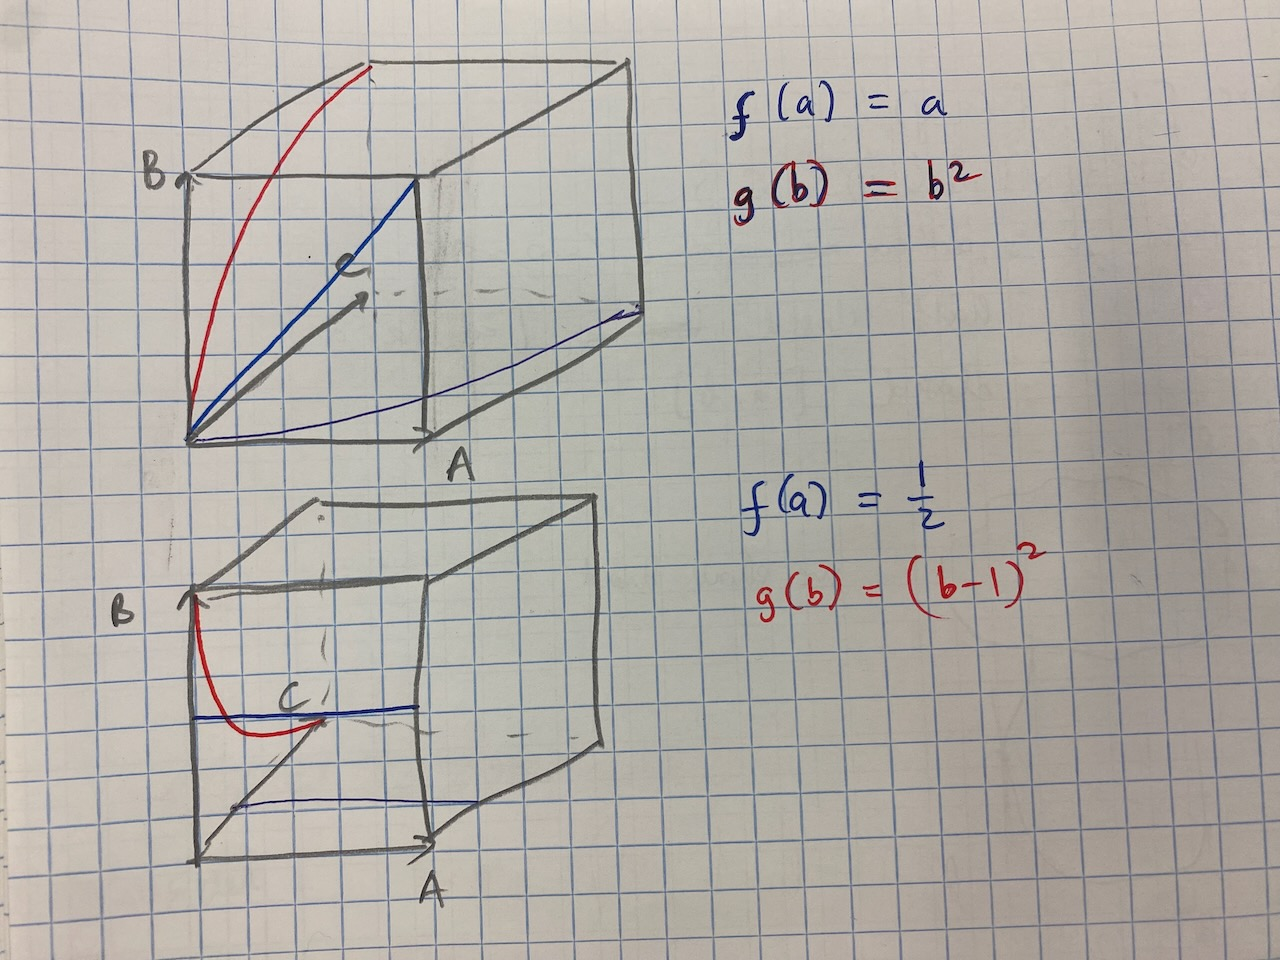
\includegraphics[width=8cm]{figures/1.21.jpeg}
    \end{center}
\end{solution}
\begin{problem} [1.22]
    A \textbf{fixed-point} of $f: A \to A$ is $a \in A$ such that $f(a) = a$. The \textbf{diagonal} of $A \times A$ is set of all pairs $(a, a)$ in $A \times A$.
    \begin{enumerate} [(a)]
        \item Show that $f: A \to A$ has a fixed point iff graph of $f$ intersects the diagonal.
        \item Prove that every continuous $f: [0,1] \to [0,1]$ has at least 1 fixed point.
        \item Is the same true for continuous $f: (0,1) \to (0,1)$?
        \item Is the same true for discontiuous functions?
    \end{enumerate}
\end{problem}

\begin{solution}
    (a) Let $S$ be the graph of $f$ and $D$ be the diagonal of $A \times A$. Then $f$ has a fixed point $\Leftrightarrow$ $\exists a \in A \:\text{such that}\: f(a) = a$ $\Leftrightarrow$ $(a, a) \in S \Leftrightarrow S \cap D \neq \emptyset$. \qed

    (b) Consider $g(x) \coloneqq f(x) - x$ defined on $[0,1]$. $f(x)$ and $x$ are continuous so $g$ is also continuous.

    We first consider cases when $f(0) = 0$ or $f(1) = 1$. Then we are done because there exists at least 1 fixed point among 0 and 1.

    We are left with when $0 < f(0), f(1) < 1$. This implies \[
    g(0) = f(0) - 0 > 0, g(1) = f(1) - 1 < 0
    \]
    so $g(1) < 0 < g(0)$.

    Since $g$ is continuous on $[0, 1]$, by IVT, $\exists c \in [0,1]$ such that $g(c) = 0 \Leftrightarrow f(c) = c$. We have found a fixed point $c$. \qed

    (c) No. Counter example: $f(x) = \frac{x + 1}{2}$ on $(0, 1)$. Then $f((0, 1)) = (1/2, 1) \subset (0, 1)$, and $f(x') = x' \implies x' = 1 \not \in (0, 1)$. \qed

    (d) No. Counter example: $f(x) = 
    \begin{cases}
        0 & \:\text{if}\: x = 1  \\
        1 & \:\text{otherwise}\: \\
    \end{cases}$
\end{solution}

\begin{problem} [1.30]
$f: (a, b) \to \bbr$ is a \textbf{convex function} if for all $x, y \in (a, b)$ and all $s, t \in [0,1]$ with $s + t = 1$ we have \[
f(sx + ty) \leq s f(x) + t f(y)
\]
\begin{enumerate} [(a)]
    \item Prove $f$ is convex iff set $S = \{(x, y): f(x) \leq y\}$ of points above its graph is convex in $\bbr^2$. 
    \item Prove that every convex function is continuous.
    \item Suppose that $f$ is convex and $a < x < u < b$. Slope $\sigma$ of the line through $(x, f(x))$ and $(u, f(u))$ depends on $x$ and $u$, say $\sigma = \sigma(x, u)$. Prove that $\sigma$ increases when $x$ increases, and $\sigma$ increases when $u$ increases.
    \item Suppose that $f$ is second-order differentiable. Prove that $f$ is convex iff $f''(x) \geq 0$ for all $x \in (a, b)$.
    \item Formulate a definition of convexity for $f: M \to \bbr$ where $M \subset \bbr^m$ is a convex set [Hint: Start with $m=2$].
\end{enumerate}
\end{problem}
\begin{solution}
    (a) \pffwd $f$ is convex.
    
    Take any $(x_0, y_0), (x_1, y_1) \in S$. We want to show $(s x_0 + tx_1, sy_0 + ty_1) \in S$ for all $s, t \in [0, 1]$ with $s + t = 1$.

    Indeed, since $f$ is convex,
    \[
    f(sx_0 + tx_1) \leq sf(x_0) + tf(x_1) \leq sy_0 + ty_1
    \]
    so $(s x_0 + tx_1, sy_0 + ty_1) \in S$

    \pfbwd $S$ is convex.
    
    Then for all $x, y \in (a, b)$, $(x, f(x)), (y, f(y)) \in S$ trivially. Since $S$ is convex, for all $s, t \in [0, 1]$ with $s+ t = 1$, $(sx + ty, sf(x) + tf(y)) \in S$ too. This implies
     \[
    f(sx + ty) \leq sf(x) + tf(y)   
    \]
    so $f$ is convex. \qed

    (b) Fix $x_0 \in (a, b)$, then choose $p = \frac{a + x_0}{2}, q = \frac{b + x_0}{2}$ so that $a < p < x_0 < q < b$.

    We first prove that $f$ is right-continuous at $x_0$. Let $x \in (x_0, q)$. Then using the convex conditions for $p < x_0 < x$ and $x_0 < x < q$, we have:
    \begin{align*}
        f(x_0) &\leq \frac{x_0 - p}{x-p}f(x) + \frac{x-x_0}{x-p}f(p) \\
        \implies \frac{x- x_0}{x-p}(f(x_0) - f(p)) & \leq \frac{x_0 - p}{x-p}(f(x) - f(x_0)) \\
        \implies f(x) - f(x_0) &\geq \frac{x-x_0}{x_0 - p}(f(x_0) - f(p))
    \end{align*}
    and
    \begin{align*}
        f(x) & \leq \frac{x- x_0}{q - x_0} f(q) + \frac{q-x}{q-x_0}f(x_0) \\
        \implies f(x) - f(x_0) &\leq \frac{x- x_0}{q-x_0} (f(q) - f(x_0))
    \end{align*}

    Therefore: \[
    \frac{x-x_0}{x_0 - p}(f(x_0) - f(p)) \leq f(x) - f(x_0) \leq \frac{x-x_0}{q-x_0}(f(q) - f(x_0))
    \]
    so $|f(x) - f(x_0)| \leq (x-x_0) \max \left\{ |\frac{f(x_0) - f(p)}{x_0 - p}|, |\frac{f(q) - f(x_0)}{q-x_0}| \right\} \leq (x-x_0) M$

    Thus for all $x_0 < x < x_0 + \frac{\epsilon}{M}$, $|f(x) - f(x_0)| < \epsilon$ so $f$ is right-continuous at $x_0$.
    
    The proof for left continuity is similar. Since $f$ is left- and right-continuous at $x_0$, $f$ is continuous at $x_0$, for all $x_0 \in (a, b)$. So $f$ is continuous on $(a, b)$. \qed

    (c) Take $x', u'$ such that $x < x' < u < u' < b$, we now prove that $\sigma(x, u) < \sigma(x', u)$ and $\sigma(x, u) < \sigma(x, u')$.

    Since $f$ is convex,
    \begin{align*}
        &f(x') \leq \frac{u- x'}{u-x} f(x) + \frac{x' - x}{u-x} f(u) \\
        &\implies \frac{u - x'}{u-x} (f(u) - f(x) ) \leq f(u) - f(x') \\
        &\implies \frac{f(u) - f(x)}{u-x} \leq \frac{f(u) - f(x')}{u-x'} \\
        &\implies \sigma(u, x) \leq \sigma(u, x')
    \end{align*}

    and \begin{align*}
        &f(u) \leq \frac{u-x}{u'- x}f(u') + \frac{u' - u}{u' - x}f(x) \\
        &\implies f(u) - f(x) \leq \frac{u-x}{u'-x}(f(u') - f(x)) \\
        &\implies \frac{f(u) - f(x)}{u - x} \leq \frac{f(u') - f(x)}{u' - x} \\
        &\implies \sigma(u, x) \leq \sigma(u', x) \qed
    \end{align*}

    (d) \pffwd $f$ is convex.

    From (c), we see that for all $ a < p < q < b$, \[
    f'(p) = \lim_{h\to 0} \sigma(p, p+h) \leq \lim_{h\to 0} \sigma(q, q + h) = f'(q)
    \]

    Therefore, with $p = x$ and $q = x + h$, \[
    f''(x) = \lim_{h \to 0+} \frac{f'(x+h) - f'(x)}{h} \geq 0 \qed
    \]

    \pfbwd $f''(x) \geq 0 \forall x \in (a, b)$.

    Since $f''(x) \geq 0 \forall x \in (a, b)$, $f'$ is an increasing function in $(a, b)$.

    We want to show that for all $x, y \in (a, b)$ and $s, t \in [0, 1]$ such that $s + t = 1$ then \[
    f(sx + ty) \leq sf(x) + t f(y)
    \]

    WLOG, suppose $x < y$ and let $p = sx + ty$. Since $f'$ is differentiable on $(a, b)$, it is integrable. Applying FTC: \[
    f(p) - f(x) = \int_{x}^{p} f'(z) dz \leq (p-x) f'(p)
    \]
    and \[
    f(y) - f(p) = \int_{p}^{y} f'(z) dz \geq (y - p) f'(p)
    \]

    so \begin{align*}
        \frac{f(p) - f(x) }{p-x} &\leq f'(p) \leq \frac{f(y) - f(p)}{y -p} \\
         f(p) (y-x) &\leq f(x)(y-p) + f(y) (p-x) \\
        f(p) &\leq f(x) \frac{y-p}{y-x} + f(y) \frac{p-x}{y-x} \\
        f(p) &\leq sf(x) + tf(y) \qed
    \end{align*}

    (e) $f: M \to \bbr$ is convex iff for all $x, y \in M$ and for all $s, t \in [0,1]$ such that $s + t = 1$, we have \[
    f(sx + ty) \leq sf(x) + t(y)
    \]

    Such a notion is well-defined, because since $M$ is convex, $\forall x, y \in M, sx + ty \in M$.
\end{solution}

\begin{problem} [1.31*]
Suppose that $f: [a, b] \to \bbr$ is monotone nondecreasing. That is, $x_1 \leq x_2 \implies f(x_1) \leq f(x_2)$.

\begin{enumerate} [(a)]
    \item Prove that $f$ is continuous except at a countable set of points. [Hint: Show that at each $x \in (a, b)$, $f$ has \textbf{right limit} $f(x+)$ and a \textbf{left limit} $f(x-)$, which are limits of $f(x + h)$ as $h \to 0$ through positive and negative values respectively. The \textbf{jump} of $f$ at $x$ is $f(x+) - f(x-)$. Show that $f$ is continuous at $x$ iff it has zero jump at $x$. At how many points can $f$ have jump $\geq 1$? At how many points can the jump be between 1/2 and 1? Between 1/3 and 1/2?]
    \item Is the same assertion true for a monotone function defined on all of $\bbr$?
\end{enumerate}
\end{problem}
\begin{solution}

    (a) Take $x \in (a, b)$. Then for any $h>0, f(x) \leq f(x +h)$ so $f(x) $ is a lower bound for $R = \{f(x+h) \mid h > 0\}$. 
    
    $R$ is non-empty, so there exists an infimum $\inf R \eqqcolon f(x+) \geq f(x)$.
    
    We prove that in fact $f(x + h) \xrightarrow{h \to 0+} f(x+)$.

    For all $\epsilon > 0$, since $f(x+) = \inf R$, there exists $\delta = \delta(\epsilon) > 0$ such that \[
    f(x+) \leq f(x + \delta) < f(x+) + \epsilon
    \]

    Then since $f(x + h)$ decreases as $h$ decreases, for all $h < \delta$ we have \[
    f(x+) \leq f(x + h) \leq f(x + \delta) < f(x+) + \epsilon
    \]
    which implies \[
    \lim_{h \to 0+} f(x + h) = f(x+)
    \]

    Similarly, there exists $\sup \{f(x+h) \mid h < 0\} \eqqcolon f(x-) \leq f(x)$ so that $\lim_{h \to 0-} f(x+h) = f(x-)$.
    
    Define $j(x) = f(x+) - f(x-)$. When $j(x) = 0$, i.e. $f(x+) = f(x-)$, the inequality $f(x-) \leq f(x) \leq f(x+)$ implies that $f(x-) = f(x) = f(x+)$, so $f$ is continuous at $x$.
    
    
    We therefore consider points $x$ where $j(x) > 0$.

    Since $f$ is monotone nondecreasing, the sum of all $j(x)$ of points $x \in (a, b)$ is at most $f(b) - f(a)$. Therefore there are at most $f(b) - f(a)$ points with $j(x) \geq 1$, at most $\frac{f(b) - f(a)}{1/2} = 2(f(b) - f(a))$ points with $1 \geq j(x) \geq 1/2, \dots$,  $(n+1)(f(b) - f(a))$ points with $1/n \geq j(x) \geq 1/(n+1) \forall n \in \bbn$.
    
    The set of points at which $j(x) > 0$ is the union of the set of points at which $1/n \geq j(x) \geq 1/(n+1)$ over all $n \in \bbn$, which is a countable union of countable sets, and is therefore countable.  \qed

    (b) Yes, it is true. Let $D_A$ be the set of discontinuity points in set $A$. Then since
    \[
    \bbr = \bigcup_{n \in \bbn} [-n, n]
    \]
    we have \[
    D_{\bbr} = \bigcup_{n \in \bbn} D_{[-n, n]}
    \]
    $D_{[-n, n]}$ is countable, so $D_{\bbr}$ is also countable.
\end{solution}

\begin{problem} [1.32*]
Suppose that $E$ is a convex region in the plane bounded by a curve $C$. \begin{enumerate} [(a)]
    \item Show that $C$ has a tangent line except at a countable number of points. [For example, a circle has a tangent line at all its points. The triangle has a tangent line except at three points, and so on.]
    \item Similarly, show that a convex function has a derivative except at a countable set of points.
\end{enumerate}
\end{problem}
\begin{solution}
    (a) We shall use part (b) to prove this.

    \textbf{Case 1: }$E$ is unbounded. 

    Then we assert that we can pick a set of axes such that there exists a function $f$ whose domain is the set of $x$-coordinates in $C$, and takes its value as corresponding $y$-coordinate of points on $C$, except at $x-$coordinates at which there are vertical lines. In which case, we define $f$ piecewise, and note that for a $x-$coordinate to have such a vertical line, it must be either the minimum value or the maximum value of the domain of $f$, therefore adding only a finite number of points without a tangent line.

    Using (b), the epigraph of (piecewise) $f$ is then convex, making it a convex function and thus only have a countable number of points without derivatives, and therefore tangent lines.

    \textbf{Case 2:} $E$ is bounded.

    Then $C$ is a closed curve.
    
    Let $D = \{x \in \bbr \mid \exists (x, y) \in C\}$, then there exists $x_{min} = \min D, x_{max} = \max D$ that has corresponding $y_{min}, y_{max}$. It does not matter which $y$ we choose, if there are multiple points on the curve of $x-$coordinate $x_{min}$.

    Draw a line connecting $(x_{min}, y_{min})$ to $(x_{max}, y_{max})$, which partitions $E$ into convex sets $E_1$ below the line and $E_2$ above the line.

    Using the current set of axes, we can then define $f: [x_{min}, x_{max}]$ that has $E_1$ as its epigraph, and reverse the direction of the $y-$axis to similarly define $g$ that has $E_2$ as its epigraph.

    Points that have vertical line can only be either $x_{min}$ or $x_{max}$, at which we can define $f$ and $g$ piecewise, only gaining a finite number of points without derivatives.

    Having convex epigraphs, $f$ and $g$ are therefore convex. Using (b), they have a countable number of points without derivatives. Combining them, there's still only a countable number of points without tangent lines. \qed

    (b) Recall that $f: (a, b) \to \bbr$ is a convex function if for all $x, y \in (a, b)$ and for all $s, t \in [0, 1]$ with $s+ t = 1$, we have \[
    f(sx + ty) \leq sf(x) + tf(y)   
    \]
    
    We have previously derived that for $u, v \in (a, b)$, \[    
        \sigma(v, u) \coloneqq \frac{f(u) - f(v)}{u-v}
    \]
    increases as $v$ increases, and also increases as $u$ increases.

    Consider a point $x_0 \in (a, b)$. We can select $p = \frac{x_0 + a}{2}, q = \frac{x_0 + b}{2}$, so that $a < p < x_0 < q < b$.

    Then we know that \[
        \sigma(p, x_0) < \sigma(x_0, x_0 + h) \forall h > 0
    \]
    so $\sigma(p, x_0)$ is a lower bound of $\{\sigma(x_0, x_0 + h) \mid h > 0 \}$. The set is non-empty, so there exists \[
        f'(x_0+) \coloneqq \inf \{\sigma(x_0, x_0 +h) \mid h > 0\}
    \]

    We shall easily prove that $\sigma(x_0, x_0 + h) \xrightarrow{h \to 0+} f'(x_0+)$. 
    
    Since $f'(x_0+)$ is the infimum, for all $\epsilon > 0$, there exists $\delta = \delta(\epsilon) > 0$ such that $f'(x_0+) \leq \sigma(x_0, x_0 + \delta) < f'(x_0+) + \epsilon$. But $\sigma(x_0, x_0 + h)$ decreases as $h$ decreases, so $\forall 0 < h < \delta$, we have \[
    f'(x_0+) \leq \sigma(x_0, x_0 + h) \leq \sigma(x_0, x_0 + \delta) < f'(x_0+) + \epsilon
    \]
    which suggests \[
        f'(x_0+) = \lim_{h \to 0+} \sigma(x_0, x_0 + h)
    \]
    is indeed the right limit of $f'$ at $x_0$.

    Similarly, there exists a left limit $f'(x_0-)$.

    It is trivial that $f'(x_0-) \leq f'(x_0+)$ based on the property of $\sigma$. So we are concerned with the number of points at which $f'(x_0-) < f'(x_0+)$  because when $f'(x_0-) = f'(x_0+)$, the derivative is defined at $x_0$.

    Let $D$ be the set of such points, then all intervals $(f'(d-) , f'(d+))$ of $d \in D$ are pairwise disjoint. Then for each interval, we are able to select a rational $Q(d) \in (f'(d-) , f'(d+))$. Then $Q: D \to \bbq$ is injective, and since $\bbq$ is countable, $D$ must be also be countable.
\end{solution}

\begin{problem} [1.48]
The trefoil cannot be unknotted in 3-space. How can you unknot the trefoil in 4-space?
\begin{center}
    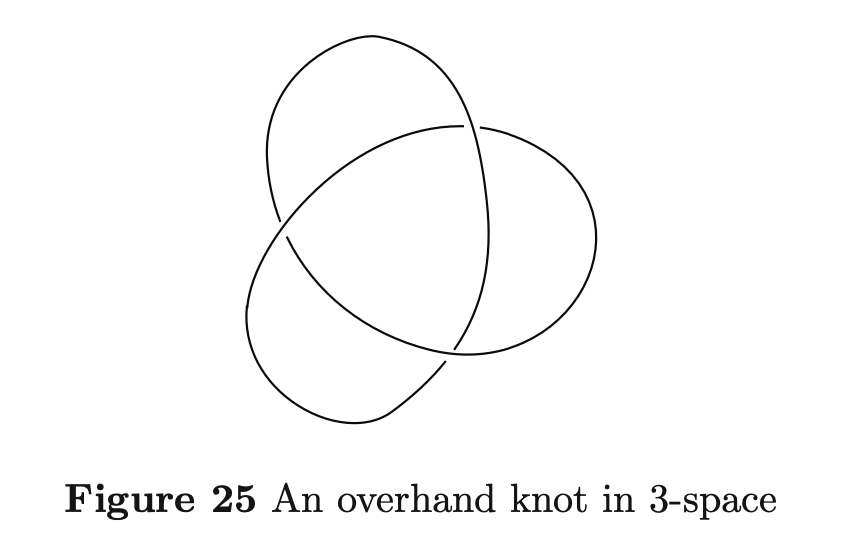
\includegraphics[width = 8cm]{figures/figure25.png}
\end{center}
\end{problem}

\begin{solution}

\mbox{}
    \begin{center}
        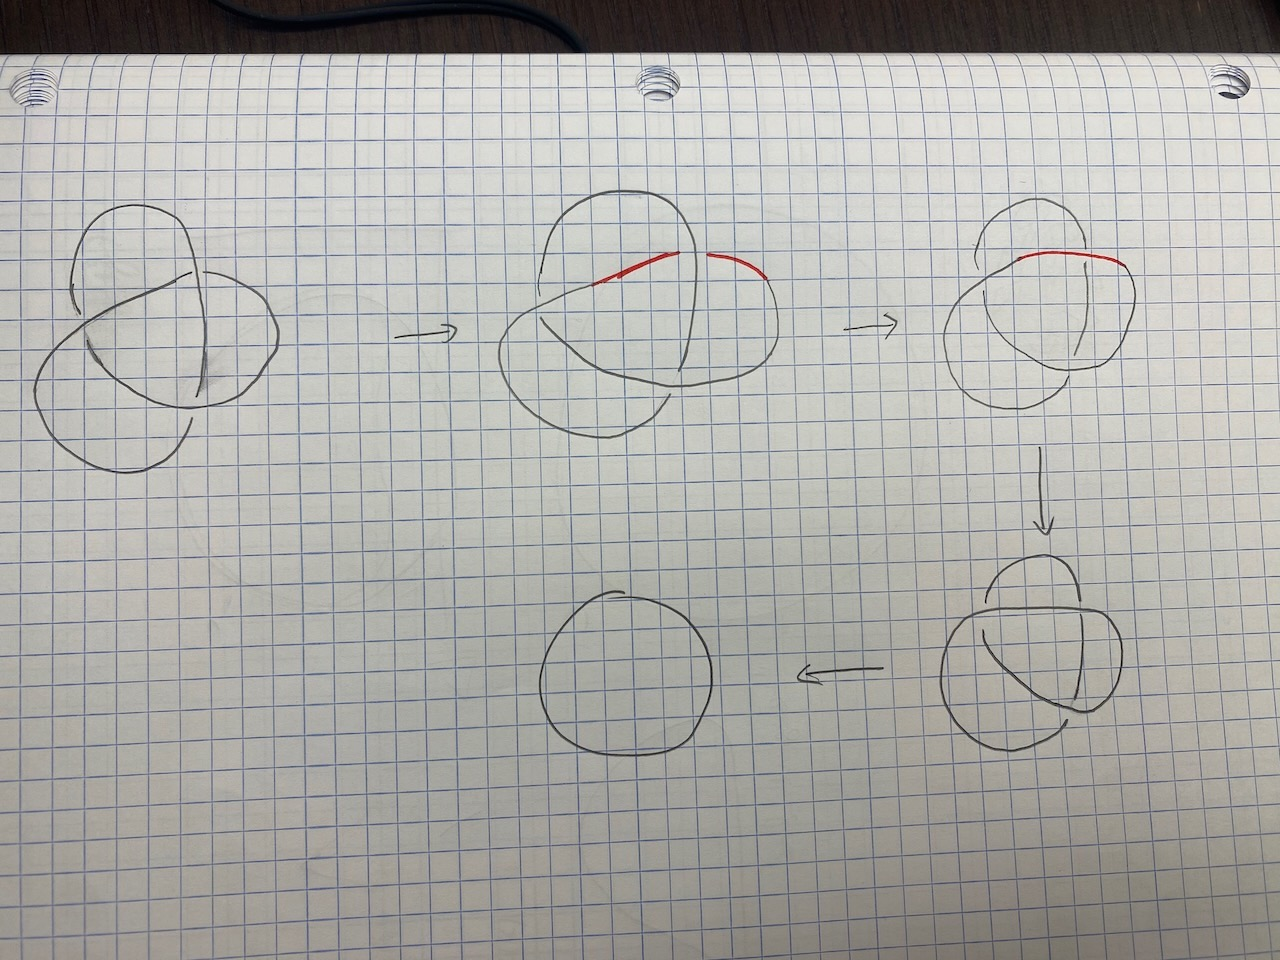
\includegraphics[width = 8cm]{figures/1.48.jpeg}
    \end{center}
\end{solution}

\begin{problem} [1.49*]
Prove that there exists no continuous three dimensional motion de-linking the two circles shown below, which keeps both circles flat at all times.
\begin{center}
    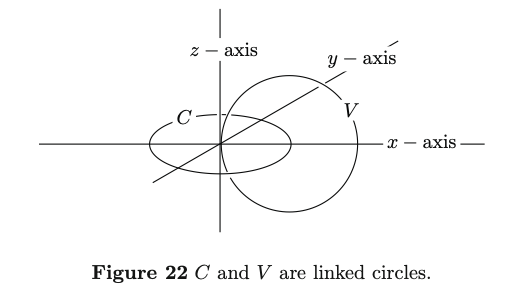
\includegraphics[width = 8cm]{figures/figure22.png}
\end{center}
\end{problem}
\begin{solution}
    My apologies for using a different set of axes.

    \begin{center}
        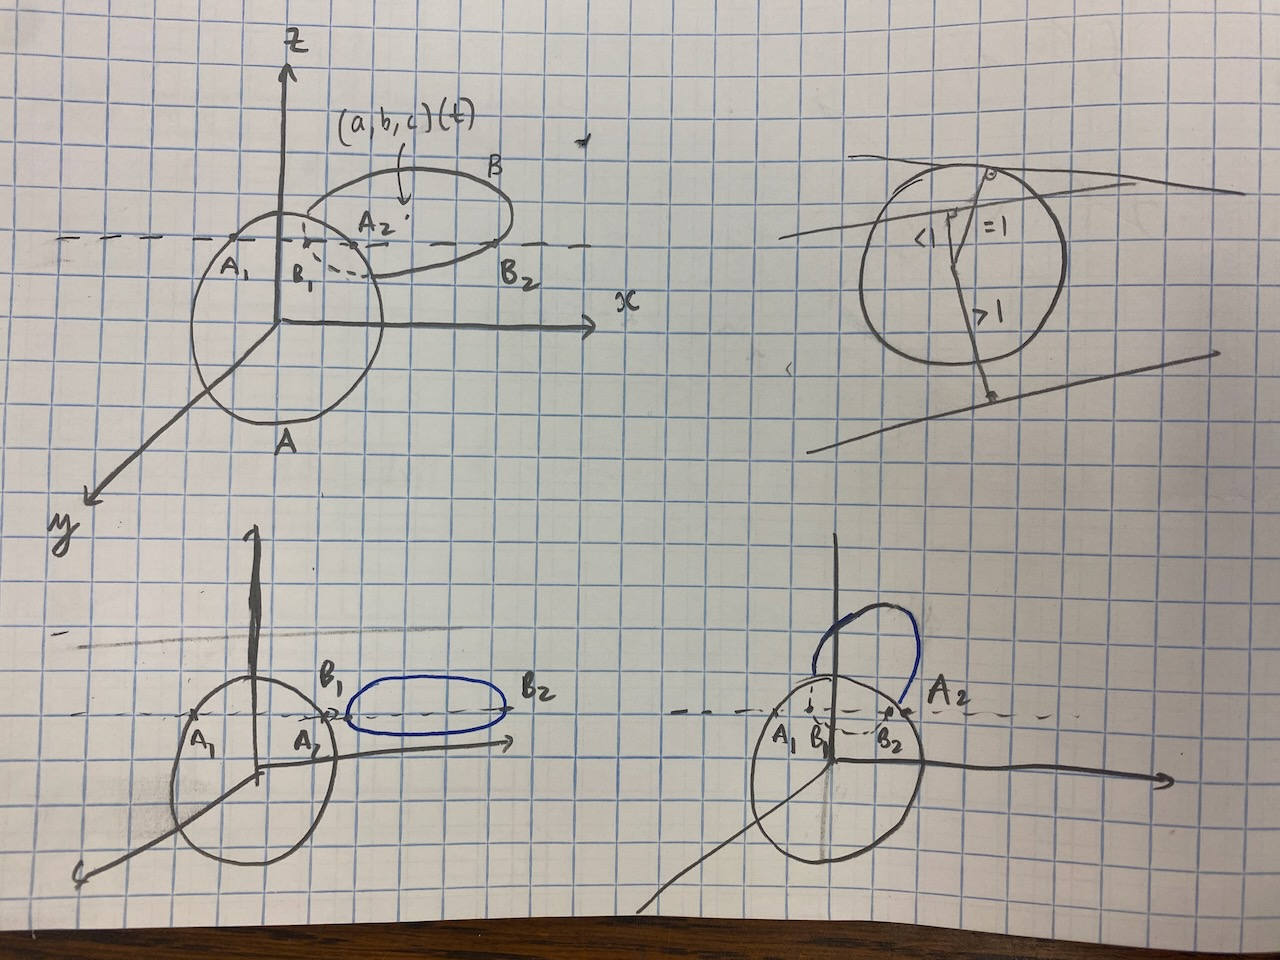
\includegraphics[width=12cm]{figures/2.49.jpeg}
    \end{center}

    WLOG, we assume that $A$ is a fixed unit circle on the $xz-$plane, centered at (0, 0, 0), and $B$ is a mobile unit circle whose movement always keeps it on a plane parallel to the $xy-$plane. WLOG, assume that when $t = 0$, $B$ is centered at (1, 0, 0). 
    
    Suppose there exists a continuous motion that delinks the 2 loops. Then if we parameterize the position of the center of $B$ as a function of time, $(a(t), b(t), c(t))$ as $t \in [0, 1]$, then $a, b, c: \bbr \to \bbr$ must also be continuous.

    Then the equation for points on $A$ is \[
        x^2 + z^2 = 1, y = 0    
    \]
    and for points on $B$ at time $t$ is \[
        (x - a(t))^2 + (z - c(t)) ^2 = 1, y = b(t)
    \]

    If the disc bounded by $A$ intersects the disc bounded by $B$, these points of intersection must lie on the line at which their 2 planes intersect, i.e. $y = 0$ and $z = c(t)$ respectively. Call this line $l$.

    Then at $t = 0$, $l$ intersects with circle $A$ at 2 points, $A_1, A_2$ and circle $B$ at 2 points, $B_1, B_2$ with the $x-$coordinate of lower-indexed points being smaller. We shall track the $x-$coordinate of these 4 points via time-dependent functions $A_1(t), A_2(t), B_1(t), B_2(t)$ until either the end of the motion, or until any of them ceases to exist (there's no longer any intersection). Since the motion is continuous, these functions shall also be continuous.

    At $t = 0, A_1(0) < B_1(0) < A_2(0) < B_2(0)$.

    As long as the 2 loops are linked, the 4 points still exist and the 4 functions still conform to this ordering, that is $B_1$ is between $A_1$ and $A_2$, and $A_2$ is between $B_1$ and $B_2$.

    When the 2 loops are de-linked, either one of the following 2 cases must happen.

    \textbf{Case 1:} There is a swapping of the aforementioned ``ABAB'' order. For example, managing to pull out $B$ in the positive $x-$ direction would yield ``AABB'' order, while squeezing $B$'s ``right'' half into $A$ would yield ``ABBA'' order. Either way, a swapping of $A_i$ and $B_j$ must have happened.

    Define $f(t) \coloneqq A_i(t) - B_j(t)$, then $f$ is continuous. But since $A_i$ and $B_j$ have swapped, either $f(0) > 0 > f(1)$ or $f(1) > 0 > f(0)$. Either case, using IVT, there exists time $t = \tau$ where $f(\tau) = 0$, $A_i$ and $B_j$ have ``merged'' into 1 point. \contra

    \textbf{Case 2:} If the order is never switched, then by the end of the motion, line $l$ as defined no longer intersects either circle $A$ or circle $B$ at any point. For example, $l$ would no longer intersect $A$ if one manages to ``lift'' $B$ up via the positive $z-$direction, after which line $l: y = 0, z = c(1) > 1$ no longer intersects $A$. $l$ would no longer intersect $B$ if one manages to ``push'' $B$ away via the negative $y-$direction, after which line $l: y = 0 >> b(1), z = c(1)$ no longer intersects $B$.

    Assume that it is the first case, where $l$ stops intersecting $A$ when $t = 1$. Let $r(t) = |c(t)|$, essentially the distance from the center of $A$ (the origin) to line $l$. It is trivial that $r$ is continuous. Here we calculate $A_1(t)$ and $A_2(t)$ in detail:
    \[
    A_1(t) = - \sqrt{1 - r(t)^2}, A_2(t) = \sqrt{1 - r(t)^2}
    \]

    At $t = 0, r(t) = 0$. When $t = 1, r(t) > 1$, since $l$ no longer intersects $A$. By IVT, there exists time $t = \tau$ such that $r(\tau) = 1$. Then, $A_1(\tau) = A_2(\tau) = 0$. But $A_1(\tau) \leq B_1(\tau) \leq A_2(\tau)$, so it must be the case that \[
        A_1(\tau) = B_1(\tau) = A_2(\tau)
    \]
    effectively meaning that $A_1, B_1$ and $A_2$ have ``merged'' into 1 point. 
    
    This is the same for when $l$ stops intersecting $B$. \contra

    Therefore, by contradiction, there exists no continuous motion that delinks the 2 circles.
\end{solution}

\begin{problem} [2.20]
What function (given by a formula) is a homeomorphism from $(-1, 1)$ to $\bbr$? Is every open interval homeomorphic to $(0, 1)$? Why or why not?
\end{problem}
\begin{solution}
    \[
    f: (0, 1) \to \bbr, f(x) = \frac{x}{\sqrt{1 - x^2}}
    \]
    is clearly continuous and bijective. Meanwhile,
    \[
        f^{-1}(y) = \frac{y}{\sqrt{y^2 + 1}}
    \]
    is continuous too. So it is a homeomorphism from $(-1, 1)$ to $\bbr$.

    Yes, every open interval $(a, b)$ is homeomorphic to $(0, 1)$. For example, we can define $g: (0, 1) \to (a, b)$ to map \[
        g(x) = a + (b-a)x
    \]
    that is clearly continuous and bijective, with inverse \[
        g^{-1}(y) = \frac{y-a}{b - a}
    \]
    is also continuous. So $g$ is a homeomorphism.
\end{solution}

\begin{problem} [2.21]
Is the plane minus four points on the $x-$axis homeomorphic to the plane minus four points in an arbitrary configuration?
\end{problem}
\begin{solution}
    Let $P_1$ be the plane minus 4 points in an arbitrary configuration. Via some linear transformation (rotation), we can select a $xy-$ coordinate system that has these 4 points at pairwise different $x-$coordinates. Let their coordinates be $\{(x_i, y_i)\}_{1 \leq i \leq 4}$.

    Let 
    \begin{multline*}
        f(x) = y_1 \frac{(x-x_2)(x-x_3)(x-x_4)}{(x_1 - x_2)(x_1 - x_3)(x_1 - x_4)} + y_2 \frac{(x-x_1)(x-x_3)(x-x_4)}{(x_2 - x_1)(x_2 - x_3)(x_2 - x_4)} + \\
        y_3 \frac{(x-x_1)(x-x_2)(x-x_4)}{(x_3 - x_1)(x_3 - x_2)(x_3 - x_4)} + y_4 \frac{(x-x_1)(x-x_2)(x-x_3)}{(x_4 - x_1)(x_4 - x_2)(x_4 - x_3)}
    \end{multline*} 
    so that $f(x_i) = y_i$ for $1 \leq i \leq 4$. Then we can transform $(x, y) \in P_1$ as follows:
    \[
    T(x, y) = (x, y - f(x))
    \]

    It is easy to see that $T$ is a bijection, there exists an inverse map that satisfies $T \circ T^{-1} = id, T^{-1} \circ T = id$, namely \[
    T^{-1} (x, y) = (x , y + f(x))
    \]

     We freely use the fact (Prof. Wilkinson) that $T$ and $T^{-1}$ are continuous. $T$ is therefore a homeomorphism. Then indeed we have $T(x_i, y_i) = (x_i, 0)$ for $ 1\leq i \leq 4$, sending our 4 original arbitrary points to 4 points on the $x-$axis.
\end{solution}

\begin{problem} [2.28]
A map $f: M \to N$ is \textbf{open} if for each open set $U \subset M$, the image set $f(U)$ is open in $N$.
\begin{enumerate} [(a)]
    \item If $f$ is open, is it continuous?
    \item If $f$ is a homeomorphism, is it open?
    \item If $f$ is an open, continuous bijection, is it a homeomorphism?
    \item If $f: \bbr \to \bbr$ is a continuous surjection, must it be open?
    \item If $f: \bbr \to \bbr$ is a continuous, open surjection, must it be a homeomorphism?
    \item What happens in (e) if $\bbr$ is replaced by the unit circle $S^1$?
\end{enumerate}
\end{problem}
\begin{solution}
    (a) No. Counter example: $f: (\bbr, d_{\bbr}) \to (\bbr, d_{discrete})$, sending $x \in [0, 1]$ to 0 and $x \in \bbr \backslash [0, 1]$ to 1. The topology induced by $d_{discrete}$ is the discrete topology, so for all open $U \subset M$, $f(U)$ is open.

    (b) Yes. Since $f$ is a homeomorphism, it bijects open sets in $M$ to open sets in $N$. Thus it sends open $U$ to open $f(U)$, so $f$ is open.

    (c) Yes, it is a homeomorphism. $f$ is already a continuous bijection, so we only need to show $f^{-1}$ is also continuous.

    i.e., $(f^{-1})^{Pre}(U)$ of open $U \subset M$ is open. Since $f$ is bijective, $(f^{-1})^{Pre}(U) = f(U)$, which is open for $U$ open because $f$ is open.

    (d) No. Counter example: \[
    f(x) = \begin{cases}
            x & \:\text{for}\: x \leq 1 \\
            2-x & \:\text{for}\: 1 \leq x \leq 2 \\
            x-2 & \:\text{for}\: x \geq 2
        \end{cases}
    \]
    then $f$ is trivially continuous, while the image set of (0, 2) is (0, 1], which is not open, so $f$ is not continuous.

    (e) Yes. We want to show that $f$ is injective.
    
    Assume there exists $x_1 \neq x_2$ such that $f(x_1) = f(x_2)$.

    Consider the image set of $[x_1, x_2]$, which by EVT and IVT, is a closed set $[m, M]$ where $m = \min_{[x_1, x_2]}f$, $M = \max_{[x_1, x_2]}f$. We consider 3 possible cases:

    \textbf{Case 1}: $m = M$, which implies that $f \equiv m$ on $[x_1, x_2]$. However this implies that the image set of $(x_1, x_2)$, an open set, is $\{m\}$, a closed set. \contra

    \textbf{Case 2}: $m \neq M$, but $f$ achieves either maximum or minimum at $x_1$     and $x_2$. WLOG, assume that $f(x_1) = f(x_2) = M$. This means that $\exists x_3 \in (x_1, x_2)$ such that $f(x_3) = m$. Then the image set of $(\frac{x_3 + x_1}{2}, \frac{x_3 + x_2}{2})$ will be a half-closed interval $[m, K)$ for some $K \in \bbr$. \contra

    \textbf{Case 3}: $m \neq M$ and $f(x_1) = f(x_2) \not \in \{m, M\}$. This means that there exists some $x_3, x_4 \in (x_1, x_2)$ such that $f(x_3) = m, f(x_4) = M$. WLOG assume $x_1 < x_3 < x_4 < x_2$, then by IVT the image set of the open interval $\left(\frac{x_1 + x_3}{2}, \frac{x_4 + x_2}{2}\right)$ is the closed interval $[m, M]$. \contra

    Therefore, by contradiction, $f$ is injective. $f$ is therefore a continuous bijection, making it a homeomorphism.

    (f) No. Parameterize points on $S^1$ as $S^1 = \{(\cos \theta, \sin \theta)\mid \theta \in [0, 2\pi)\}$. Then define $f: S^1 \to S^1$ as \[
    f((\cos \theta, \sin \theta)) = (\cos 2\theta, \sin 2\theta)
    \]
    then $f$ is clearly continuous (we travel around $S^1$ twice as fast). $f$ is also open, and surjective ($f((\cos \theta/2, \sin \theta/2)) = (\cos \theta, \sin \theta)$ for all $\theta \in [0, 2\pi) $), but $f$ is not injective ($f((\cos 0, \sin 0)) = f((\cos \pi, \sin \pi)) = (1, 0)$) so it can't be a homeomorphism.
\end{solution}
\end{document}
